\chapter{Modelling of the Battlefield}
\label{ch:modelling}
As expressed in the introduction, this thesis wants to be innovative in 2 ways:
\begin{enumerate}
    \item Create a mathematical model of the battlefield that can be used for simulation on a computer.
    \item Assess whether state-of-the-art MARL techniques are able to develop interesting strategies in the framework of this model.
\end{enumerate}
In this chapter, we will develop a simple and a more complex model of the battlefield.  Chapter \ref{ch:impl_eval} will evaluate how the algorithms of the previous chapter interact with these models.\\
A mathematical - or algorithmic - model has two goals:
\begin{enumerate}
    \item To make explicit which simplifications we'll make, both about the terrain itself as about the agents that interact on this terrain.
    \item To allow a computer to manipulate the model, simulate different situations and predict their outcomes.
\end{enumerate}
An important question is which level of detail we aspire to. As in all simulations, this must be a trade-off between making something as simple as possible to reduce computational complexity, and retain enough details to make it realistic and useful. To work towards this equilibrium, two versions of the model were developed with increasing level of complexity.\\
A model consists of two parts:
\begin{enumerate}
    \item The \emph{environment}, which contains the terrain and imposes the rules of the game. The environment keeps at all times a global state of the game which encapsulates all relevant knowledge about the current situation. The rules of the game determine which actions are allowed in which circumstances and what the next state $s'$ will be when an action $a$ is taken in a state $s$. The environment thus implements the transition probability $p(s'|s, a)$. It also provides a reward for each agent.
    \item The \emph{agents} that are present. Agents will be part of a \emph{team}, in our case team "\textcolor{blue}{blue}" and team "\textcolor{red}{red}". Only the agents of team blue are learning agents. The agents interact with the environment through their actions and receive observations.
\end{enumerate}
This formalism is completely in line with the reinforcement learning paradigm as sketched in figure \ref{fig:mdp}. At the same time, all forms of the game subscribe to the multi-agent formalism for Markov games, as defined in section \ref{sec:intro_marl}.

%---------------------------------------------------------------------------------------
\section{Initial Model}
\label{sec:first_model}
Two opposing teams \emph{blue} and \emph{red} play against each other. Each team consists of two agents, which we'll consider to be tanks. The game is played on a flat terrain without obstacles. The size of the game board is small, typically $7$ by $7$.\\
This game offers perfectly symmetrical capabilities to both teams: every tank $T_i$ is the same and has following individual state vector $s^i_t$:
\begin{enumerate}
    \item a position $(x,y)$ on the board,
    \item a boolean value {\tt alive} that determines whether the agent in question is still alive,
    \item an integer {\tt ammo} that specifies how many shots an agent has left,
    \item an integer {\tt aim} that specifies whether the agent is aiming at one of the opposing agents.
\end{enumerate}
The global state $\bm{s_t}$ is then a tuple $(s_t^0, s_t^1, s_t^2, s_t^3) \in \bm{S}$ with $\bm{S}$ the set of global states.\\
Each agent can choose among $8$ actions:
\begin{enumerate}
    \item {\tt do\_nothing}\\
        As the name says, the agent does nothing and its state vector $s^i$ doesn't change.
    \item {\tt aim0} \\
        Aims at the first tank of the opposing player and thus changes the {\tt aim} variable of its state vector. The agent must be alive to be able to execute this action.
    \item {\tt aim1} \\
        Idem as above but aiming at the second tank of the opposing player.
    \item {\tt fire} \\
        Fire at the tank the agent is aiming at. This decreases the {\tt ammo} counter. The agent must be alive, have sufficient ammo and must be aiming before executing this action.\\
        If the opposing tank is in range (determined by a parameter {\tt max\_range}), its {\tt alive} indicator will be set to {\tt False}. This means that every shot will result in a killed opponent if in range.
    \item 4 {\tt move} actions ({\tt north}, {\tt south}, {\tt east}, {\tt west})\\
        The agent will move one step in the desired direction, unless he will drop of the board or tries to move to a tile occupied by an other agent.
        %or comes too close to another agent\footnote{This is done to avoid that two agents will end up in the same spot since actions are, in the general case, executed simultaneously and if agents are too close, they can move to the same square.}.
\end{enumerate}

The joint action space $\mathcal{A}$ thus consists of all tuples of actions $(a_t^0, a_t^1, a_t^2, a_t^3)$ whereby the first two actions are executed by agents belonging to player $P_0$ and the two others by agents of $P_1$. Actions are executed simultaneously. A player loses when both his tanks are dead or out of ammo. While the out-of-ammo criterion is a realistic assumption, it also avoids long games without end and thus speeds up learning. Additionally, a small penalty is introduced for every step an agent takes. This should induce an agent to prefer shorter episodes. Experience has shown that this addition does indeed shorten the average game time and speeds up learning compared to the situation without penalty. Additionally, at the reset of a game, all agents are placed in the same initial position.\\
All agents receive an observation from the environment that is based on the global state vector. An observation $o^i_t$ for agent $i$ consists of the following information:
\begin{itemize}
    \item His own position, remaining ammo and, if applicable, the opposing agent he is aiming at.
    \item The relative position of his team mate and of the opposing agents, if they are still alive.
\end{itemize}
This implies that an agent does not know the ammo situation of other agents nor if any of the opposing agents is aiming and at whom. This is a design choice to mimic a realistic situation.\\
An advantage of this kind of representation is that it is defined from the view point of the agent itself thanks to e.g. the choice to communicate the position of others relative to the agents own position. This will allow us to share networks among agents from the same which greatly increases sample efficiency and transferability of models, two advantages that will be discussed in chapter \ref{ch:impl_eval}.\\
Figure \ref{fig:game_visual} shows a standard visualization of the game, where tanks of the blue team are both dead (they are "greyed out").

\begin{figure}[htp]
    \centering
    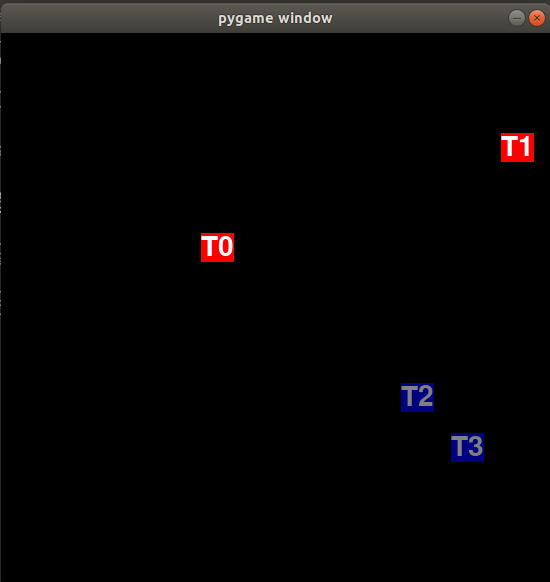
\includegraphics[width=8cm]{images/game_visual.png}
    \caption{Visualization of the simple version of the game}
    \label{fig:game_visual}
\end{figure}



%---------------------------------------------------------------------------------------
\section{Extended Model}
\label{sec:extended_model}
The goal of extending the model is to make it more realistic while still keeping it manageable. Several extensions to the simple model have been considered. These proposed extensions include:
\begin{enumerate}
    \item Using asymmetric agents with different capabilities (e.g. tanks vs. warriors with RPG).
    \item More than 2 vs. 2 agents.
    \item Complex terrain where both visibility and mobility are blocked by obstacles.
    \item Larger state space, where e.g. fuel is limited.
    \item More complex firing probability, e.g. an exponentially decreasing probability based on distance between shooter and target.
\end{enumerate}
Since time for this thesis was limited, only the second and third option were retained; the others will be explored in future research.\\
This means that the second model is a model where the agents all have the same capabilities as before but the number of agents of both teams can be chosen freely and is not limited. Furthermore, we'll take into account the terrain which consists of free space and obstacles.\\
Since the number of opposing agents increases, the number of actions available to an agent also increases. A part from {\tt do\_nothing}, {\tt fire} and the {\tt move}-actions, the agent can now chose to aim at any opponent on the board. This is a minor change but it implies that the size of the action-space is no longer fixed which in turn has implications for the RL algorithms.\\
Obstacles in the terrain block both the movement and the line-of-sight of the agents. A blocked line-of-sight means that firing is not allowed, although aiming is still possible.\\
Just as before, each agent receives an observation from the environment which is derived from the global state. The agent receives information about:
\begin{itemize}
    \item His own position, ammo and who he's aiming at.
    \item The relative position of the other agents.
\end{itemize}
This observation is extended with:
\begin{itemize}
    \item Information about which tiles contain an obstacle and this for the entire board.
    \item Information about which enemy agent is visible and can thus be fired at. 
\end{itemize}
The environment thus uses the terrain information to inform an agent whether the opposing agents are visible. The agent is aware of the entire terrain, even the parts that are not visible. This is a deviation from reality and this shortcoming will be addressed in future research.\\
This environment model, together with the models for agents, actions, observations and states, can be found in \url{https://github.com/koenboeckx/VKHO/blob/master/env.py}.